\documentclass[tikz, border=2pt]{standalone}
\usepackage{amsmath}

\begin{document}
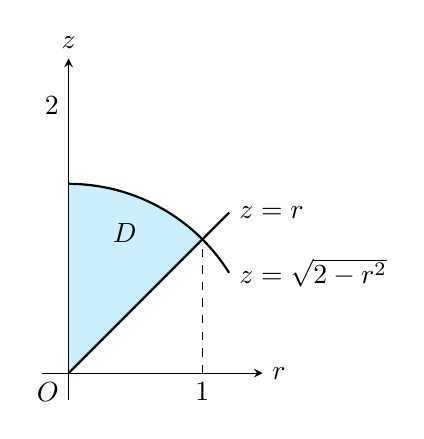
\begin{tikzpicture}[scale=1.7, >=stealth]
    % Cross-section in the rz-plane: r <= z <= sqrt(2-r^2).
    \fill[cyan!20]
    (0,0)
    -- plot[domain=0:1, samples=80] (\x,{\x})
    -- plot[domain=1:0, samples=100] (\x,{sqrt(2-\x*\x)})
    -- cycle;

    \draw[->] (-0.2,0) -- (1.45,0) node[right] {$r$};
    \draw[->] (0,-0.2) -- (0,2.35) node[above] {$z$};

    \draw[thick, domain=0:1.2, samples=80] plot (\x,{\x}) node[right] {$z=r$};
    \draw[thick, domain=0:1.2, samples=100] plot (\x,{sqrt(2-\x*\x)}) node[right] {$z=\sqrt{2-r^2}$};
    \draw[dashed] (1,0) node[below] {$1$} -- (1,1);

    \node[below left] at (0,0) {$O$};
    \node[left] at (0,2) {$2$};
    \node at (0.42,1.05) {$D$};
\end{tikzpicture}
\end{document}
